\documentclass{article}
\usepackage{tikz}

\begin{document}

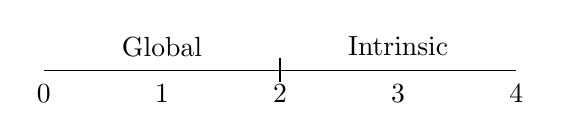
\begin{tikzpicture}[scale=1.5]
    % Draw the horizontal line
    \draw (0,0) -- (4,0);
    
    % Break the line at x=2
    \draw[thick] (2,-0.1) -- (2,0.1);
    
    % Label the segments
    \node at (1,0.2) {Global};
    \node at (3,0.2) {Intrinsic};
    
    % Add some numbers along the line
    \foreach \x/\y in {0/0, 1/1, 2/2, 3/3, 4/4} {
        \node at (\x,-0.2) {\y};
    }
\end{tikzpicture}

\end{document}